\documentclass{standalone}

\usepackage{tikz}
\usetikzlibrary{arrows}
\usetikzlibrary{decorations.markings}
\usepackage{standalone}

\begin{document}

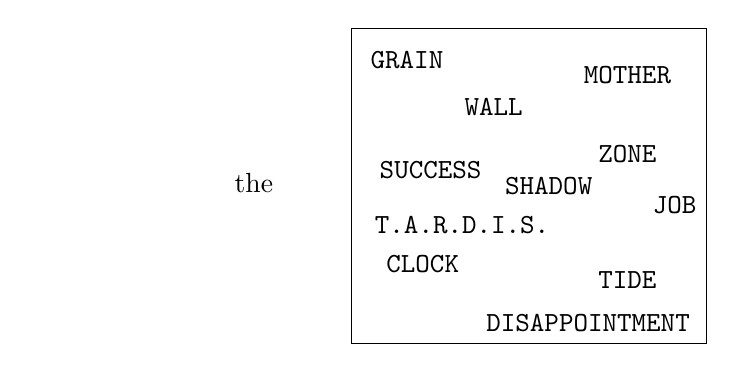
\begin{tikzpicture}


\node[text width=3cm, align=right] at (0, 6) {\textcolor{white}{race against} the};

\draw (2.5, 4) rectangle (7, 8);

\node at (3.4, 5) {\texttt{CLOCK}};
\node at (3.2, 7.6) {\texttt{GRAIN}};
\node at (6, 4.8) {\texttt{TIDE}};
\node at (4.3, 7) {\texttt{WALL}};
\node at (6.6, 5.75) {\texttt{JOB}};
\node at (5.5, 4.25) {\texttt{DISAPPOINTMENT}};
\node at (6, 6.4) {\texttt{ZONE}};
\node at (6, 7.4) {\texttt{MOTHER}};
\node at (5, 6) {\texttt{SHADOW}};
\node at (3.9, 5.5) {\texttt{T.A.R.D.I.S.}};
\node at (3.5, 6.2) {\texttt{SUCCESS}};



\end{tikzpicture}

\end{document}
